\documentclass[UTF8]{ctexart}
\usepackage{booktabs}  % professionally typeset tables
\usepackage{amsmath}
\usepackage{setspace}
\usepackage{textcomp}  % better copyright sign, among other things
\usepackage{xcolor}
\usepackage{lipsum}    % filler text
\usepackage{subfig}   
\usepackage{geometry}
\usepackage{float}
\usepackage{hyperref}
\usepackage{graphicx}


\geometry{left=2.54cm,right=2.54cm,top=2.18cm,bottom=3.18cm}
\date{}
\title{\textbf{竞赛讲座管理系统设计文档}}
\author{\rightline{SigmaGo小组}} 


\begin{document}
%\begin{CJK}{UTF8}{gbsn}
\begin{spacing}{1.3}
\maketitle


\section{简介}

\subsection{系统简介}
针对于校园中讲座和竞赛资源的流通性不足、同学们获取信息和资源的方式过于分散等问题,我们小组希望能够设计一个竞赛讲座管理系统,通过对于竞赛、讲座等信息进行统一整理和总结,并且设计一种算法对于特定同学进行合适的讲座和竞赛的推荐,增加同学们对于自己所需要的讲座、感兴趣的竞赛的认知,从而实现信息的最大化利用。

\subsection{系统功能}
略

\subsection{目标用户}
略

\section{系统框架(类图)}

\subsection{功能模块}
		\begin{figure}[H]
				\centering
				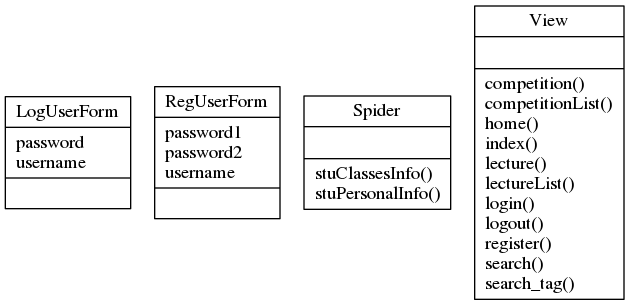
\includegraphics[width=\textwidth]{classes_view.png}
		\end{figure}

\subsection{数据库模块}
		\begin{figure}[H]
				\centering
				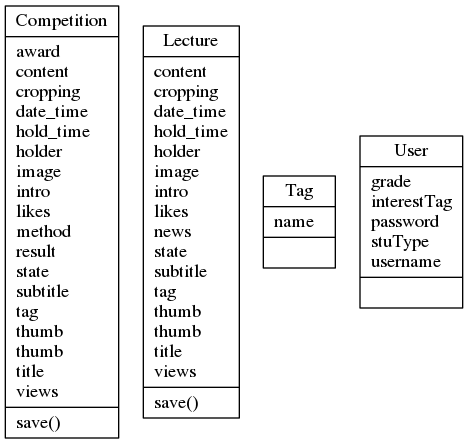
\includegraphics[width=\textwidth]{classes_model.png}
		\end{figure}

%\section{实验收获与小结}
%\section{程序来源说明}
\end{spacing}
\end{document}
